The COLDATA ASIC is responsible for all communication between the cold TPC electronics on FEMBs and electronics located outside the cryostat.  The COLDATA ASIC is being designed by engineers from Fermilab and Southern Methodist University.  Each FEMB contains two COLDATA ASICs.  COLDATA receives command and control information; it provides clocks to the Cold ADC ASICs and relays commands to the LArASIC front-end and to the Cold ADC ASICs to set operating modes and initiate calibration procedures.  COLDATA receives data from the ADC ASICs, reformats these data, merges data streams, formats data packets, and sends these data packets to the warm electronics using 1.28 Gbps links.  These links include line drivers with pulse preemphasis.  All the components of COLDATA, with the exception of the line drivers and of the interface to the ADC, have been implemented in the CDP1 prototype ASIC and demonstrated to work as designed both at room temperature and at 77~K.  A block diagram of COLDATA is shown in Figure~\ref{fig:coldata}.  

\begin{dunefigure}
[Block diagram of COLDATA ASIC design.]
{fig:coldata}
{Block diagram of COLDATA ASIC design.}
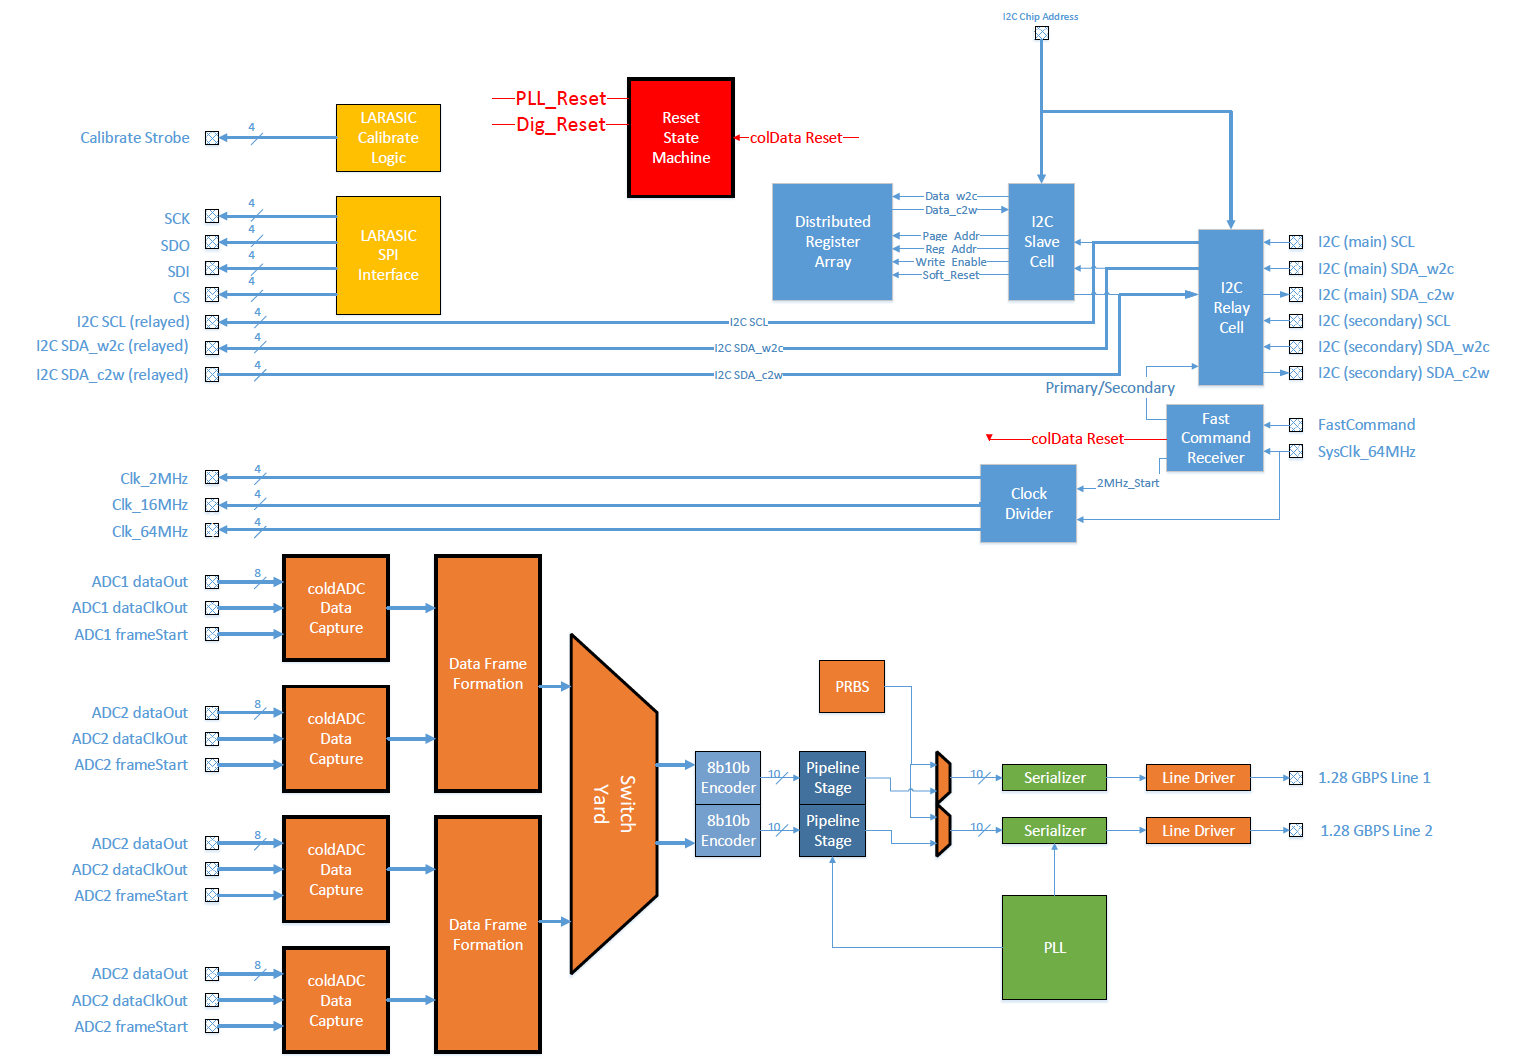
\includegraphics[width=0.9\linewidth]{tpcelec-COLDATABlockDiagram.png}
\end{dunefigure}

Both COLDATA and Cold ADC are implemented in TSMC 65 nm CMOS using ``cold'' transistor models produced by Logix, Consulting.  Logix made measurements of Fermilab-supplied TSMC 65~nm transistors at a variety of temperatures (including room temperature and liquid nitrogen temperature).  They extracted and provided to Fermilab SPICE models as a function of temperature.  A special library of standard cells, based on these SPICE models and using a minimum channel length of 90 nm, was developed by members of the University of Pennsylvania and Fermilab groups.  This library was designed to eliminate the risk posed by the hot carrier effect.  The digital sections of COLDATA and Cold ADC use these standard cells and were synthesized from RTL using automatic place and route tools.
